\section{Design / Implementation}
\label{ch:impl}
\noindent	

This chapter aims to discuss the implementation details of the system presented in \textit{figure~\ref{system-overview}}.

\subsection{CoAP server}

\begin{figure}[H]
	\begin{center}
		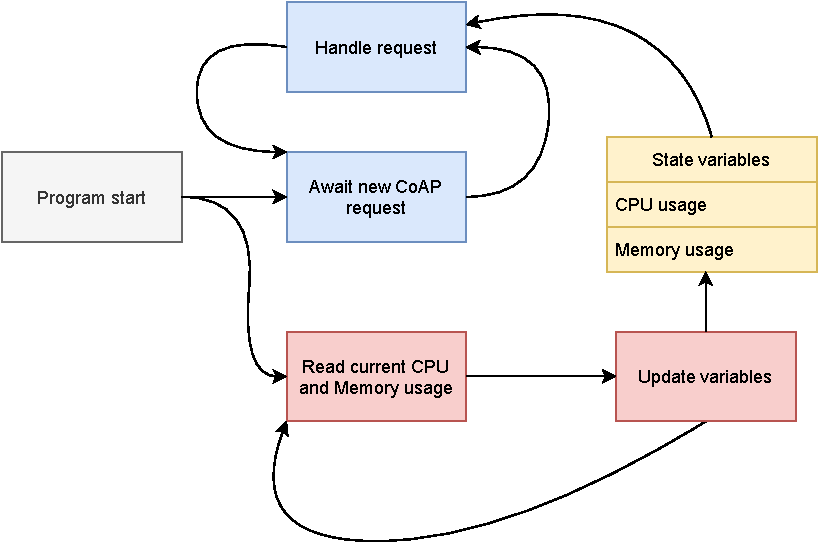
\includegraphics[width=\textwidth]{./doc/coap_flowchart.pdf}
		\caption{Flowchart depicting the duties and the program flow of the CoAP server.}
		\label{coap-figure}
	\end{center}
\end{figure}

\subsection{CoAP + MQTT Client}

\textit{Figure~\ref{coap-figure}} shows the program flow of the CoAP server. The flow is separated into two threads marked as blue and red boxes in figure~\ref{coap-figure}. There is also a yellow box, representing data shared between the threads. This data is locked behind mutex locks so as to not cause any race conditions between the red and blue thread. 

The red thread is responsible for regularly reading the current CPU and memory usage from the system. It then tries to access the shared state variables in order to update them with the new information. Upon successfully updating the variables, the lock is released and the thread sleeps for one second before attempting to read the CPU and memory usage once more.

The blue thread is responsible for performing all server-related duties of the system component. It listens for potential requests to the urls \lstinline{/cpu} and \lstinline{/mem}. Upon recieving a request, it tries to access the corresponding shared state variable, embeds it into a response, and sends the response. It then goes back into listening mode, awaiting the next request.

\subsection{MQTT Broker}

\subsection{MQTT Client + WebSocket server}

\subsection{HTML/JS frontend}

\iffalse
The Design or Implementation chapter often appears in technical reports, but not always in scientific reports. Here, the analysis of the problem is implemented and a technical requirement specification is formulated. At this stage, the most important principles in the suggested alternatives for solution are described and formulated in preparation for evaluation at a later point in the report. The description is sometimes placed before, but generally after the methodology/model chapter, if included at all.

The reader is seldom interested in extremely detailed documentation of computer program code, algorithms, electrical circuit diagrams, user guidance, etc. Such details are placed in the appendices.

As mentioned in the Introduction chapter you have during earlier studies mainly worked with small well defined tasks that have taken minutes or as most hours to solve. In comparison an exam work or a project course can sometimes appear to be an almost overwhelming amount of information because it is so extensive, and this may cause anxiety with regards to where to start. One way to facilitate big projects is to use the top-down-method, i.e. to divide the problem or the structure into smaller problem parts or system parts, and to state specification of  requirements, problem analysis and proposed solution for each part. Eventually small and concrete information will have been identified with similar characteristics to those found in your previous studies.

It is not always practically possible to apply the top-down-method, since the problem may be too complex and initially very difficult to visualise the complete overview. It might prove necessary to alternate between the top-down - and bottom-up-method. The latter means that you start with parts already known to you and from simple problems that have been tackled previously you  make use of that knowledge for aspects that you expect to resolve at a later stage in the project. Gradually increase these parts into the bigger systems and problems and then pursue the direction of project's objective.

The top-down-method has the advantage of giving the report a solid structure, which makes it easier for the reader. The documentation therefore often follows the top-down-method. It is thus possible to divide the structure part into several chapters, and to name them after each problem part and system part, i.e. “Specification of requirements”, “Algorithms”, “User interface”, “Program documentation”, “Prototype” and “Implementation”.
\fi
